\subsection{Le cas primitif}

Les exemples 9 à 12 donnés en annexe B illustrent les propositions,
définitions et théorèmes de cette section.

\begin{prop}
    Puisque $\mathcal{PF'}_n$ et $\mathcal{D}_n$ ont le même cardinal,
    nous pouvons créer une \emph{bijection} entre les fonctions de parking
    classiques primitives de longueur $n$ et les mots de Dyck de
    longueur $2n$.
\end{prop}

\begin{proof}
    ~\
\begin{itemize}
    \item $\mathcal{PF'}_n \to \mathcal{D}_n$ :
    Soit $f = (a_1, \ldots, a_n) \in \mathcal{PF'}_n$
    une fonction de parking classique primitive.
    Pour tout $i \in \{1, \ldots, n\}$, notons $l_i$ le nombre
    d'occurences de $i$ dans $f$.\\
    Le mot de Dyck correspondant sera alors
    $\underbrace{1 \cdots 1}_{l_1}0
     \underbrace{1 \cdots 1}_{l_2}0 \cdots
     \underbrace{1 \cdots 1}_{l_n}0$.
    
    \item $\mathcal{D}_n \to \mathcal{PF'}_n$ :
    Soit $w \in \mathcal{D}_n$ un mot de Dyck. Considérons sa
    représentation sous la forme d'un chemin de Dyck.
    Notons $s_i$ l'abscisse du $i^{e}$ pas Nord.
    On pose alors $a_i = s_i + 1$.\\
    La fonction de parking primitive correspondante sera ainsi
    $(a_1, \ldots, a_n)$.
\end{itemize}
\end{proof}

Nous proposons maintenant des relations de couverture pour ces deux
ensembles, telles que les posets ainsi créés soient isomorphes, et que 
l'un puisse être obtenu en appliquant la bijection ci-dessus à l'autre.

\begin{definition}[$\gtrdot_d$]
    Soient $w$ et $w'$ deux mots de Dyck de longueur $2n$.
    On dit que $w$ couvre $w'$, noté $w \gtrdot_d w'$, s'il existe deux
    mots $w_1$ et $w_2$ tels que :
    \begin{itemize}
        \item $w = w_101w_2$
        \item $w' = w_110w_2$
    \end{itemize}  
\end{definition}

\begin{rem}
    Si $w_1 \gtrdot_d w_2$, alors le chemin de Dyck correspondant à $w_2$
    est \emph{au dessus} de celui correspondant à $w_1$, et La
    \emph{différence} entre les deux chemins est un carré de côté 1.
\end{rem}

\begin{definition}[Chemins de Dyck Imbriqués]
    Deux chemins de Dyck $w_1$ et $w_2$ sont dits \emph{imbriqués}
    si $w_1$ est égal à $w_2$ ou au dessus de $w_2$. 
\end{definition}

On déduit donc la proposition suivante de la remarque précédente.

\begin{prop}
    IS'il existe une séquence $w_1 \gtrdot_d w_2 \gtrdot_d
    w_3 \gtrdot_d \cdots \gtrdot_d w_k$ avec $k \geqslant 0$,
    alors $w_1$ et $w_k$ sont \emph{imbriqués}.
\end{prop}

Cette relation de couverture engendre notre \emph{poset} pour
$\mathcal{D}_n$.
Ainsi, le poset contient l'\emph{intervalle} $[w_1;w_2]$ si et seulement
si $w_1$ et $w_2$ sont imbriqués.

On définit maintenant la relation bijective sur les fonctions de parking.
Celle-ci sera la même pour les 4 types de fonctions de parking (classiques,
classiques primitives, rationnelles, et rationnelles primitives).

\begin{definition}[$\gtrdot$]
    Soient $f$ et $g$ deux fonctions de parking.
    On dit que $f$ couvre $g$, noté $f \gtrdot g$, s'il existe $i$ tel que :
    \begin{itemize}
        \item $f = (a_1, \ldots, a_{i-1}, a_i,\ \ \ \ 
            a_{i+1}, \ldots, a_n)$
        \item $g = (a_1, \ldots, a_{i-1}, a_i - 1, a_{i+1},
        \ldots, a_n)$
    \end{itemize}
\end{definition}

Cette relation de couverture engendre notre poset pour $\mathcal{PF'}_n$.

\begin{theorem}[Théorème principal]
    Le nombre d'intervalles dans ces posets est égal au $n+1^{e}$ terme
    de la suite de l'OEIS 
    \href{https://oeis.org/A005700}{A005700}
    \footnote{https://oeis.org/A005700}.\\
    Alec Mihailovs a démontré que le $n^{e}$ terme de cette séquence est
    égal à $$\frac {6 (2n)! (2n+2)!}{n!(n+1)!(n+2)!(n+3)!}$$.
\end{theorem}

Les premiers termes de cette suite sont $1, 1, 3, 14, 84,
594, 4719, 40898, 379236, 3711916, ...$\\

\begin{proof}
    Puisque le nombre d'intervalles dans le poset de $\mathcal{D}_n$
    peut être vu comme le nombre de paires $(w_1, w_k)$ telles que
    $w_1 \gtrdot_d w_2 \gtrdot_d \cdots \gtrdot_d w_k$, alors nous pouvons
    décrire le nombre d'intervalles comme étant le nombre de 
    \emph{paires de chemins de Dyck imbriqués}.
    Ce nombre est bien égal à la suite A005700 (Bruce Westbury, 2013).
\end{proof}

\begin{expl}[Les posets de $\mathcal{D}_4$ et $\mathcal{PF'}_4$]
    ~\\
    \begin{center}
        \begin{center}
    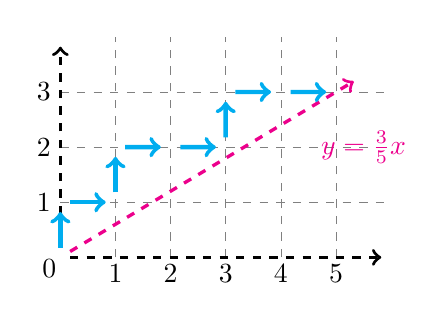
\begin{tikzpicture}[scale=0.7]
        \node (a) at (0, 0) {};
        \node (b) at (0, 4) {};
        \node (c) at (6, 0) {};
        \node (d) at (5.5, 3.3) {};

        \draw [dashed, very thin, color=gray] (1,0) to (1,4);
        \draw [dashed, very thin, color=gray] (2,0) to (2,4);
        \draw [dashed, very thin, color=gray] (3,0) to (3,4);
        \draw [dashed, very thin, color=gray] (4,0) to (4,4);
        \draw [dashed, very thin, color=gray] (5,0) to (5,4);
        \draw [dashed, very thin, color=gray] (0,1) to (6,1);
        \draw [dashed, very thin, color=gray] (0,2) to (6,2);
        \draw [dashed, very thin, color=gray] (0,3) to (6,3);
        
        \node (e) at (5.5, 2) [color = magenta] {$y = \frac{3}{5}x$}; 
        \draw [dashed, very thick, ->] (a) to (b);
        \draw [dashed, very thick, ->] (a) to (c);
        \draw [dashed, very thick, ->]
            [color = magenta] (a) to (d);

        \node (1)  at (0,0)   {};
        \node (2)  at (0,1)   {};
        \node (3)  at (1,1)   {};
        \node (4)  at (1,2)   {};
        \node (5)  at (2,2)   {};
        \node (6)  at (3,2)   {};
        \node (7)  at (3,3)   {};
        \node (8)  at (4,3)   {};
        \node (9)  at (5,3)   {};
        \draw [->, ultra thick, color = cyan]
            (1)  to (2);
        \draw [->, ultra thick, color = cyan] 
            (2)  to (3);
        \draw [->, ultra thick, color = cyan]
            (3)  to (4);
        \draw [->, ultra thick, color = cyan]
            (4)  to (5);
        \draw [->, ultra thick, color = cyan]
            (5)  to (6);
        \draw [->, ultra thick, color = cyan]
            (6)  to (7);
        \draw [->, ultra thick, color = cyan]
            (7)  to (8);
        \draw [->, ultra thick, color = cyan]
            (8)  to (9);

        \node at (-0.2, -0.2) {$0$};
        \node at (-0.3, 1)    {$1$};
        \node at (1, -0.3)    {$1$};
        \node at (-0.3, 2)    {$2$};
        \node at (2, -0.3)    {$2$};
        \node at (-0.3, 3)    {$3$};
        \node at (3, -0.3)    {$3$};
        \node at (4, -0.3)    {$4$};
        \node at (5, -0.3)    {$5$};

    \end{tikzpicture}
\end{center}
        Ces posets contiennent chacun $\frac {1}{5} \binom{8}{4} =
        14$ éléments et $84$ relations.
    \end{center}
\end{expl}

On souhaite maintenant étendre cette construction au cas non-primitif.
Bien que celle sur les fonctions de parking soit la même, il
reste à expliciter la bijection, et à définir la relation de couverture
sur les mots de Dyck \emph{décorés}.

\subsection{Le cas général}

Les exemples 13 à 16 donnés en annexe B illustrent les propositions,
définitions et théorèmes de cette section.

\begin{prop}
    Puisque $\mathcal{PF}_n$ et $\mathcal{LD}_n$ ont le même cardinal,
    nous pouvons créer une \emph{bijection} entre les fonctions de parking
    classiques de longueur $n$ et les mots de Dyck décorés de
    longueur $2n$.
\end{prop}

\begin{proof}
    ~\
    \begin{itemize}
        \item $\mathcal{PF}_n \to \mathcal{LD}_n$ :
        Soit $f = (a_1, \ldots, a_n) \in \mathcal{PF}_n$ une fonction de
        parking. Pour tout $i \in \{1, \ldots, n\}$, posons $im_i$ :
        $\{j\ |\ a_j = i\}$. \\
        Notons alors $im_{i,1}, \ldots, im_{i,k_i}$ les éléments de $im_i$
        triés par ordre croissant.\\
        Le mot de Dyck décoré correspondant sera 
        $\underbrace{im_{1,1} \cdots im_{1,k_1}}_{im_1}0
         \underbrace{im_{2,1} \cdots im_{2,k_2}}_{im_2}0
         \cdots
         \underbrace{im_{n,1} \cdots im_{n,k_n}}_{im_n}0$.

        \item $\mathcal{LD}_n \to \mathcal{PF}_n$ :
        Soit $w$ un mot de Dyck décoré. Considérons sa représentation sous
        la forme d'un chemin de Dyck. Notons $s_i$ l'abscisse du $i^{e}$ pas
        Nord.\\
        On note alors $label(i)$ le label du $i^{e}$ pas nord, et
        $dist_i = \{label(j) | s_j = i\}$ l'ensemble  des labels des pas
        Nord à distance $i$ de l'axe des ordonnées.\\
        Ainsi, si $j \in dist_i$, on pose $a_j = i + 1$.\\
        La fonction de parking correspondante sera donc $(a_1, \ldots, a_n)$.
    \end{itemize}
\end{proof}

La relation suivante est l'extension de $\gtrdot_d$ au cas décoré.

\begin{definition}[$\gtrdot_{ld}$]
    Soient $w$ et $w'$ deux mots de Dyck décorés. On dit que $w$ couvre
    $w'$, noté $w \gtrdot_{ld} w'$, s'il existe $l$, $r$, $x$, $x'$, $y$,
    $z$, et $z'$ tels que :
    \begin{itemize}
        \item $l$ est le mot vide, ou finit par un $0$
        \item $r$ est le mot vide, ou commence par un $0$
        \item $x = x_1x_2 \cdots$ avec $x_i > 0$ pour tout $i$
        \item $z = z_1z_2 \cdots$ avec $z_i > 0$ pour tout $i$
        \item $x' = x$ où $y$ est correctement inséré en ordre croissant
        \item $y$ apparait dans $z$, et $z' = z$ où $y$ à été supprimé
        \item $w = lx0zr$
        \item $w' = lx'0z'r$
    \end{itemize}
\end{definition}

Pour expliquer l'idée derrière cette relation de couverture, nous aurons
besoin de la définition suivante.

\begin{definition}[Montée]
    Une \emph{montée} d'un mot de Dyck (décoré ou non) est une sous-mot
    maximal ne contenant pas de 0, et suivi d'un 0.
\end{definition}

\begin{rem}
    Si $w_1 \gtrdot_{ld} w_2$, alors le chemin de Dyck décoré correspondant
    à $w_2$ est \emph{au dessus} de celui correspondant à $w_1$,
    et la \emph{différence} entre les deux est un carré de côté 1.\\
    De plus, la relation $\gtrdot_{ld}$ peut être vue ainsi :
    $w_1$ couvre $w_2$ si et seulement si l'on peut obtenir $w_2$ à partir
    de $w_1$ en enlevant un élément de la $i + 1^{e}$ montée, 
    et en réinsérant cet élément en ordre croissant dans la $i^{e}$
    montée.
\end{rem}

Cette relation de couverture engendre notre poset pour $\mathcal{LD}_n$.
En gardant la relation $\gtrdot$ sur l'ensemble des fonctions de parking
classiques, on obtient ainsi les posets bijectifs espérés.


\begin{conj}[Conjecture Principale]
    Le nombre d'intervalles des posets définis ici pour $\mathcal{LD}_n$
    et $\mathcal{PF}_n$ est le $n+1^{e}$ terme de la suite de l'OEIS
    \href{https://oeis.org/A196304}{A196304}
    \footnote{https://oeis.org/A196304}.
\end{conj}

Les premiers termes de cette suite sont $1, 1, 5, 64, 1587,
65421, 4071178, 357962760, 4237910716, ...$.

\begin{expl}[Les posets de $\mathcal{LD}_3$ et $\mathcal{PF}_3$]
    ~\\
    \begin{center}
        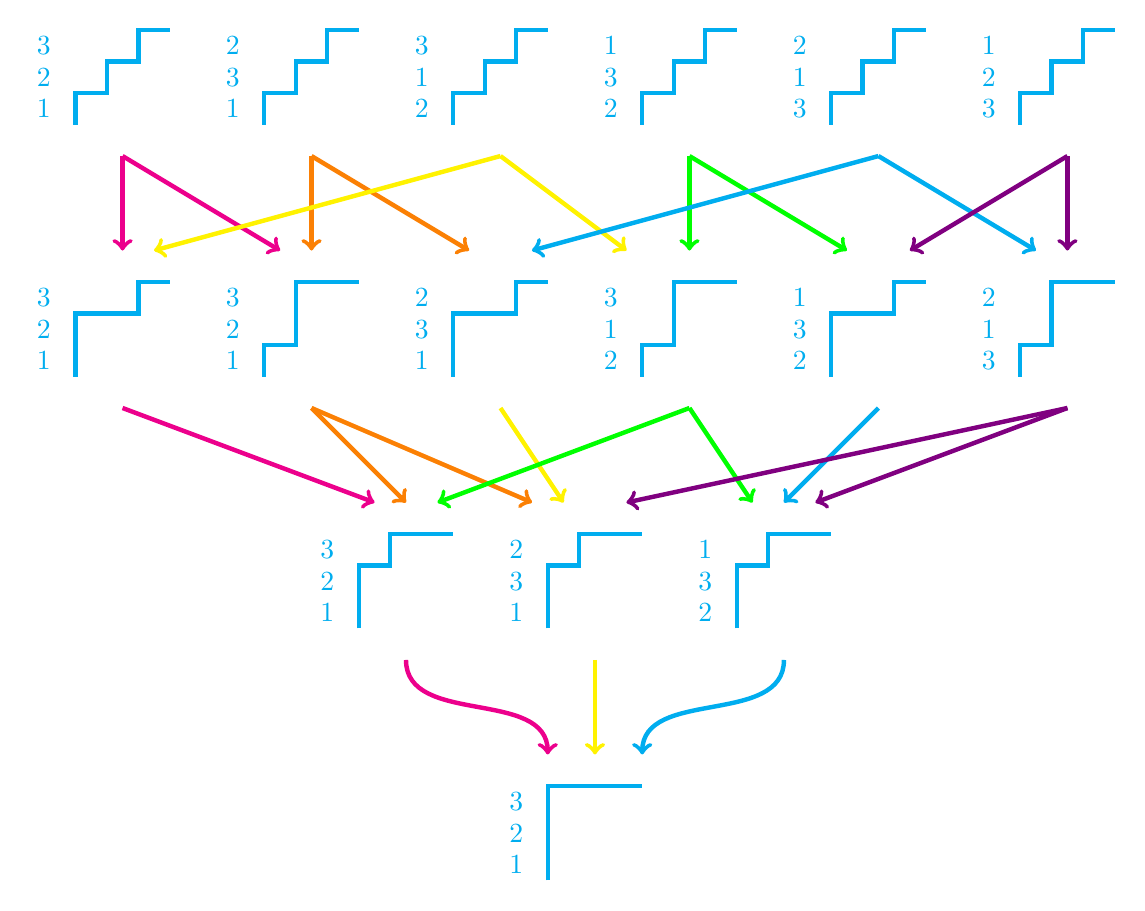
\begin{tikzpicture}[scale = 0.4]
    \draw [ultra thick, color = cyan] (0,0) -- (0,1)
        -- (0,2) -- (0,3) -- (1,3) -- (2,3) -- (3,3);
    \node[color = cyan] at (-1,0.5) {$1$};
    \node[color = cyan] at (-1,1.5) {$2$};
    \node[color = cyan] at (-1,2.5) {$3$};

    \draw [ultra thick, color = cyan] (-6,8) -- (-6,9)
        -- (-6,10) -- (-5,10) -- (-5,11) -- (-4,11)
        -- (-3,11);
    \node[color = cyan] at (-7,8.5) {$1$};
    \node[color = cyan] at (-7,9.5) {$2$};
    \node[color = cyan] at (-7,10.5) {$3$};
        
    \draw [ultra thick, color = cyan] (0,8) -- (0,9)
        -- (0,10) -- (1,10) -- (1,11) -- (2,11)
        -- (3,11);
    \node[color = cyan] at (-1,8.5) {$1$};
    \node[color = cyan] at (-1,9.5) {$3$};
    \node[color = cyan] at (-1,10.5) {$2$};

    \draw [ultra thick, color = cyan] (6,8) -- (6,9)
        -- (6,10) -- (7,10) -- (7,11) -- (8,11)
         -- (9,11);
    \node[color = cyan] at (5,8.5) {$2$};
    \node[color = cyan] at (5,9.5) {$3$};
    \node[color = cyan] at (5,10.5) {$1$};

    \draw [ultra thick, color = cyan] (-15,16) -- (-15,17)
        -- (-15,18) -- (-14,18) -- (-13,18) -- (-13,19)
        -- (-12,19);
    \node[color = cyan] at (-16,16.5) {$1$};
    \node[color = cyan] at (-16,17.5) {$2$};
    \node[color = cyan] at (-16,18.5) {$3$};

    \draw [ultra thick, color = cyan] (-9,16) -- (-9,17)
        -- (-8,17) -- (-8,18) -- (-8,19) -- (-7,19)
        -- (-6,19);
    \node[color = cyan] at (-10,16.5) {$1$};
    \node[color = cyan] at (-10,17.5) {$2$};
    \node[color = cyan] at (-10,18.5) {$3$};

    \draw [ultra thick, color = cyan] (-3,16) -- (-3,17)
        -- (-3,18) -- (-2,18) -- (-1,18) -- (-1,19)
        -- (0,19);
    \node[color = cyan] at (-4,16.5) {$1$};
    \node[color = cyan] at (-4,17.5) {$3$};
    \node[color = cyan] at (-4,18.5) {$2$};

    \draw [ultra thick, color = cyan] (3,16) -- (3,17)
        -- (4,17) -- (4,18) -- (4,19) -- (5,19)
        -- (6,19);
    \node[color = cyan] at (2,16.5) {$2$};
    \node[color = cyan] at (2,17.5) {$1$};
    \node[color = cyan] at (2,18.5) {$3$};

    \draw [ultra thick, color = cyan] (9,16) -- (9,17)
        -- (9,18) -- (10,18) -- (11,18) -- (11,19)
        -- (12,19);
    \node[color = cyan] at (8,16.5) {$2$};
    \node[color = cyan] at (8,17.5) {$3$};
    \node[color = cyan] at (8,18.5) {$1$};

    \draw [ultra thick, color = cyan] (15,16) -- (15,17)
        -- (16,17) -- (16,18) -- (16,19) -- (17,19)
        -- (18,19);
    \node[color = cyan] at (14,16.5) {$3$};
    \node[color = cyan] at (14,17.5) {$1$};
    \node[color = cyan] at (14,18.5) {$2$};

    \draw [ultra thick, color = cyan] (-15,24) -- (-15,25)
        -- (-14,25) -- (-14,26) -- (-13,26) -- (-13,27)
        -- (-12,27);
    \node[color = cyan] at (-16,24.5) {$1$};
    \node[color = cyan] at (-16,25.5) {$2$};
    \node[color = cyan] at (-16,26.5) {$3$};

    \draw [ultra thick, color = cyan] (-9,24) -- (-9,25)
        -- (-8,25) -- (-8,26) -- (-7,26) -- (-7,27)
        -- (-6,27);
    \node[color = cyan] at (-10,24.5) {$1$};
    \node[color = cyan] at (-10,25.5) {$3$};
    \node[color = cyan] at (-10,26.5) {$2$};

    \draw [ultra thick, color = cyan] (-3,24) -- (-3,25)
        -- (-2,25) -- (-2,26) -- (-1,26) -- (-1,27)
        -- (0,27);
    \node[color = cyan] at (-4,24.5) {$2$};
    \node[color = cyan] at (-4,25.5) {$1$};
    \node[color = cyan] at (-4,26.5) {$3$};


    \draw [ultra thick, color = cyan] (3,24) -- (3,25)
        -- (4,25) -- (4,26) -- (5,26) -- (5,27)
        -- (6,27);
    \node[color = cyan] at (2,24.5) {$2$};
    \node[color = cyan] at (2,25.5) {$3$};
    \node[color = cyan] at (2,26.5) {$1$};

    \draw [ultra thick, color = cyan] (9,24) -- (9,25)
        -- (10,25) -- (10,26) -- (11,26) -- (11,27)
        -- (12,27);
    \node[color = cyan] at (8,24.5) {$3$};
    \node[color = cyan] at (8,25.5) {$1$};
    \node[color = cyan] at (8,26.5) {$2$};

    \draw [ultra thick, color = cyan] (15,24) -- (15,25)
        -- (16,25) -- (16,26) -- (17,26) -- (17,27)
        -- (18,27);
    \node[color = cyan] at (14,24.5) {$3$};
    \node[color = cyan] at (14,25.5) {$2$};
    \node[color = cyan] at (14,26.5) {$1$};

    \draw [->][color=magenta, ultra thick]
        (-13.5,23) to (-13.5,20);
    \draw [->][color=magenta, ultra thick]
        (-13.5,23) to (-8.5,20);
    \draw [->][color=magenta, ultra thick]
        (-13.5,15) to (-5.5,12); 
    \draw [->][out=-90,in=90, ultra thick] 
        [color=magenta](-4.5,7) to (0,4);

    \draw [->][color=brown!7!orange, ultra thick]
        (-7.5,23) to (-7.5,20);
    \draw [->][color=brown!7!orange, ultra thick]
        (-7.5,23) to (-2.5,20);
    \draw [->][color=brown!7!orange, ultra thick]
        (-7.5,15) to (-4.5,12);
    \draw [->][color=brown!7!orange, ultra thick]
        (-7.5,15) to (-0.5,12);

    \draw [->][color=yellow, ultra thick]
        (-1.5,23) to (-12.5,20);
    \draw [->][color=yellow, ultra thick]
        (-1.5,23) to (2.5,20);
    \draw [->][color=yellow, ultra thick]
        (-1.5,15) to (0.5,12); 
    \draw [->][out=-90,in=90, ultra thick] 
        [color=yellow](1.5,7) to (1.5,4);

    \draw [->][color = green,  ultra thick]
        (4.5,23) to (4.5,20);
    \draw [->][color=green, ultra thick]
        (4.5,23) to (9.5,20);
    \draw [->][color=green, ultra thick]
        (4.5,15) to (-3.5,12);
    \draw [->][color=green, ultra thick]
        (4.5,15) to (6.5,12);

    \draw [->][color=cyan, ultra thick]
        (10.5,23) to (-0.5,20);
    \draw [->][color=cyan, ultra thick]
        (10.5,23) to (15.5,20);
    \draw [->][color=cyan, ultra thick]
        (10.5,15) to (7.5,12); 
    \draw [->][out=-90,in=90, ultra thick] 
        [color=cyan](7.5,7) to (3,4);

    \draw [->][color=violet, ultra thick]
        (16.5,23) to (11.5,20);
    \draw [->][color=violet, ultra thick]
        (16.5,23) to (16.5,20);
    \draw [->][color=violet, ultra thick]
        (16.5,15) to (2.5,12);
    \draw [->][color=violet, ultra thick]
        (16.5,15) to (8.5,12);

\end{tikzpicture}

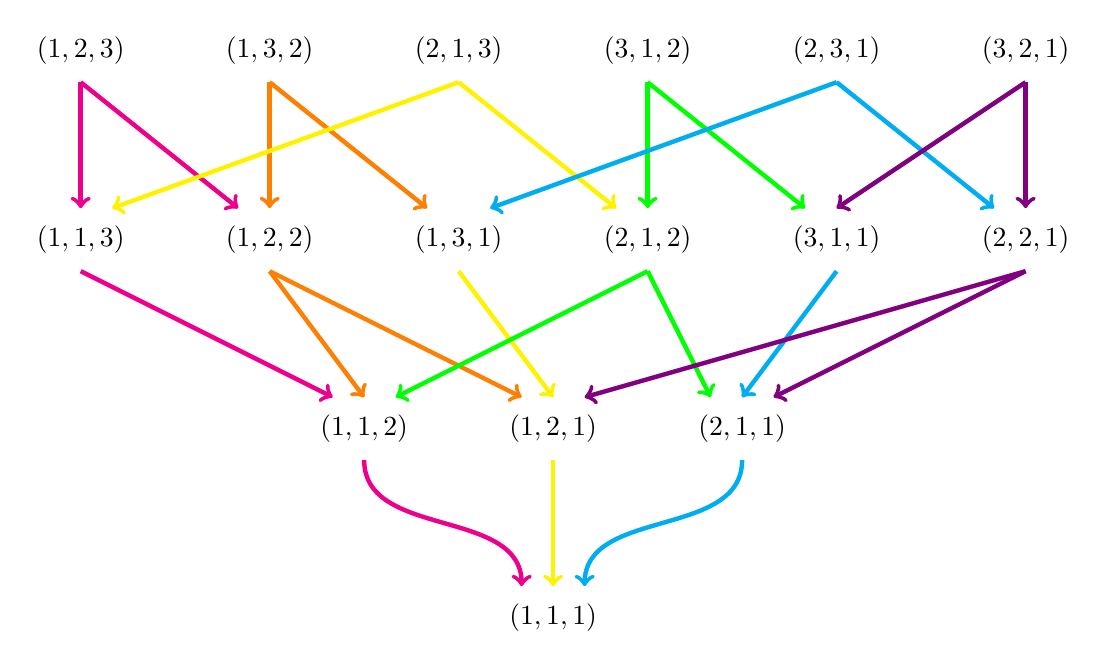
\begin{tikzpicture}[scale = 0.4]
    \node at (0,0) {$(1,1,1)$};

    \node at (-6,6) {$(1,1,2)$};                
    \node at (0,6)  {$(1,2,1)$};
    \node at (6,6)  {$(2,1,1)$};

    \node at (-15,12) {$(1,1,3)$};
    \node at (-9,12)  {$(1,2,2)$};
    \node at (-3,12)  {$(1,3,1)$};
    \node at (3,12)   {$(2,1,2)$};
    \node at (9,12)   {$(3,1,1)$};
    \node at (15,12)  {$(2,2,1)$};

    \node at (-15,18) {$(1,2,3)$};
    \node at (-9,18)  {$(1,3,2)$};
    \node at (-3,18)  {$(2,1,3)$};
    \node at (3,18)   {$(3,1,2)$};
    \node at (9,18)   {$(2,3,1)$};
    \node at (15,18)  {$(3,2,1)$};

    \draw [->][color=magenta, ultra thick]
        (-15,17) to (-15,13);
    \draw [->][color=magenta, ultra thick]
        (-15,17) to (-10,13);
    \draw [->][color=magenta, ultra thick]
        (-15,11) to (-7,7); 
    \draw [->][out=-90,in=90, ultra thick] 
        [color=magenta](-6,5) to (-1,1);

    \draw [->][color=brown!7!orange, ultra thick]
        (-9,17) to (-9,13);
    \draw [->][color=brown!7!orange, ultra thick]
        (-9,17) to (-4,13);
    \draw [->][color=brown!7!orange, ultra thick]
        (-9,11) to (-6,7);
    \draw [->][color=brown!7!orange, ultra thick]
        (-9,11) to (-1,7);

    \draw [->][color=yellow, ultra thick]
        (-3,17) to (-14,13);
    \draw [->][color=yellow, ultra thick]
        (-3,17) to (2,13);
    \draw [->][color=yellow, ultra thick]
        (-3,11) to (0,7); 
    \draw [->][out=-90,in=90, ultra thick] 
        [color=yellow](0,5) to (0,1);

    \draw [->][color = green,  ultra thick]
        (3,17) to (3,13);
    \draw [->][color=green, ultra thick]
        (3,17) to (8,13);
    \draw [->][color=green, ultra thick]
        (3,11) to (-5,7);
    \draw [->][color=green, ultra thick]
        (3,11) to (5,7);

    \draw [->][color=cyan, ultra thick]
        (9,17) to (-2,13);
    \draw [->][color=cyan, ultra thick]
        (9,17) to (14,13);
    \draw [->][color=cyan, ultra thick]
        (9,11) to (6,7); 
    \draw [->][out=-90,in=90, ultra thick] 
        [color=cyan](6,5) to (1,1);

    \draw [->][color=violet, ultra thick]
        (15,17) to (9,13);
    \draw [->][color=violet, ultra thick]
        (15,17) to (15,13);
    \draw [->][color=violet, ultra thick]
        (15,11) to (1,7);
    \draw [->][color=violet, ultra thick]
        (15,11) to (7,7);

\end{tikzpicture}
~\\
~\\
        Il y a $4^2 = 16$ éléments et $64$ intervalles dans chacun de ces
        posets.
    \end{center}
\end{expl}

Bien que, à notre connaissance, il n'existe pas de structure combinatoire
associée à cette suite, les tests effectués via Sagemath sur
$n = 1, 2, \cdots, 8$ suggèrent que le nombre d'intervalles de nos posets
puissent en être une.\\

Pour aller plus loin, la prochaine partie aborde une généralisation des
fonctions de parking : les fonctions de parking \emph{rationnelles}.

Cette extension peut être vue ainsi :
Soit $(a_1, \ldots, a_n)$ une séquence d'entiers positifs,
et $(b_1, \ldots, b_n)$ son tri par ordre croissant.
Dans le cas classique, les limites pour $(b_1, \ldots, b_n)$
étaient $(1, \ldots, n)$, et dépendaient donc d'un unique entier $n$.
Dans le cas rationnel, les limites dépendront de \emph{deux entier
premiers entre eux} $a$ et $b$.
Plus précisément, ces limites seront $(1, 1 + \frac{b}{a},
1 + \frac{2b}{a}, 1 + \frac{3b}{a}, \ldots)$, avec $a = n$. 